\documentclass[11pt]{article}

% Build from this directory with:
%   pdflatex WHITEPAPER.tex
%   pdflatex WHITEPAPER.tex
%
% The document intentionally uses LaTeX's default Computer Modern typeface.
\usepackage{amsmath}
\usepackage{array}
\usepackage{tikz}
\usepackage[hidelinks]{hyperref}
\usepackage{url}
\usetikzlibrary{arrows.meta,positioning}
\hypersetup{
  pdftitle={Coppice Names: Private, Trustless Names on Zcash},
  pdfsubject={Draft whitepaper, version 0.1}
}

\newcommand{\operation}[1]{\texttt{#1}}
\newcommand{\statusword}[1]{\textbf{#1}}
\newcommand{\code}[1]{\texttt{#1}}
\setlength{\emergencystretch}{1em}

\title{Coppice Names:\\Private, Trustless Names on Zcash}
\author{}
\date{Draft whitepaper, version 0.1\\September 2026}

\begin{document}

\maketitle

\begin{abstract}
Coppice Names is a privacy-preserving naming protocol built entirely on the
current Zcash transaction and shielded-note model. It maps a short
\code{.zec} name to a canonical Zcash Unified Address without adding a
sidechain, consensus change, trusted name server, global registry operator, or
protocol-specific token. Each registration is backed by an exact 1 ZEC
shielded note that remains under its owner's control. The owner's authority
stays hidden, and releasing a name is an ordinary spend that returns the bond,
less the normal Zcash transaction fee.

The protocol combines a name-hiding \operation{COMMIT}, a scheduled
name-routed \operation{REVEAL}, and a proof-carrying \operation{REFRESH}
operation. Zero-knowledge proofs establish hidden ownership and bond-note
transitions, while a deterministic reducer applies public timing, ordering,
lineage, and spentness rules against the canonical Zcash chain. Any wallet can
resolve an arbitrary exact name by deriving its public route, authenticating
the referenced historical \operation{COMMIT}, and replaying the name's
accepted lineage. A rolling cache of canonical compact Zcash evidence makes
this process fast without turning a local index into an authority.

On a retained 250,000-block Orchard-family mainnet workload containing 688,370
actions, the production wallet-position replay path processed the Coppice and
Names components in 1.853 seconds. The duplicate-tree reference path took
239.52 seconds on the same workload, a measured 99.23\% reduction. This is an
isolated in-memory replay result, not an end-to-end resolution latency promise;
network acquisition, database persistence, live Coppice transactions, and
production proof workloads remain to be qualified.
\end{abstract}

\section*{Status of this document}

Coppice Names is implemented but not deployed. This document presents the
intended protocol as one coherent design. It is an explanatory whitepaper, not
the normative protocol definition; implementations must follow the protocol
specification and its conformance artifacts.

\begin{center}
\small
\begin{tabular}{>{\raggedright\arraybackslash}p{0.55\textwidth}p{0.30\textwidth}}
\hline
Area & Status \\
\hline
Protocol construction and deterministic reducer & Implemented \\
\operation{REVEAL} and \operation{REFRESH} circuits & Implemented; exercised by conformance vectors \\
Exact-name resolver and wallet integration & Implemented \\
Six-month replay performance study & Preliminary; measured and modeled as labelled \\
Independent cryptographic review & WIP \\
End-to-end deployment qualification & WIP \\
Production deployment parameters and activation & TBD \\
\hline
\end{tabular}
\end{center}

Statements marked \statusword{WIP}, \statusword{TBD},
\statusword{measured}, or \statusword{modeled} retain those qualifiers until
the corresponding work is complete.

\section{Motivation}

Cryptocurrency addresses are precise but difficult for people to recognize,
remember, and verify. A naming layer can improve payment usability, but a
conventional naming service often introduces an operator, an externally
trusted index, public ownership records, or a separate consensus system. Those
choices are especially costly for a privacy-oriented currency.

Coppice Names begins from five requirements:

\begin{enumerate}
\item A resolver must be able to resolve any exact name, not only names it
previously followed.
\item Correctness must come from Zcash's canonical transaction history and
locally verified protocol rules, not from a trusted third-party answer.
\item Registration authority and the bonded note should remain shielded.
\item The registrant must retain ownership of the bond; registration must
neither burn ZEC nor transfer it to a protocol operator.
\item The construction must fit within current Zcash consensus and transaction
capabilities.
\end{enumerate}

The result is an application protocol carried by Zcash transactions. Zcash
provides transaction validity, canonical ordering, shielded-note semantics,
and fork choice~\cite{zcash-protocol,zip258}. Coppice provides authenticated
application publication and replay. Coppice Names adds name-specific proofs
and deterministic state rules.

\subsection{Non-goals}

Coppice Names does not attempt to provide:

\begin{itemize}
\item ownership transfer between hidden authorities;
\item fuzzy, prefix, or directory search as a consensus feature;
\item permanent names without renewal;
\item free transaction publication;
\item a trusted remote resolver or hosted index; or
\item a Names state root committed by Zcash consensus.
\end{itemize}

Wallets may build local search interfaces over derived state, but such indexes
are conveniences rather than resolution authority.

\section{System and trust model}

The system has four principal roles:

\begin{itemize}
\item A \emph{registrant} controls a Zcash wallet, a hidden per-name authority,
and an exact 1 ZEC Ironwood note used as the bond.
\item A \emph{resolver} derives public name routes and independently evaluates
Names operations found in canonical Zcash history.
\item A \emph{wallet host} authenticates compact and full transaction data,
maintains canonical scan state, handles reorganizations, and protects managed
bond notes from accidental ordinary spending.
\item The \emph{Zcash network} validates and orders transactions and supplies
the underlying shielded-note state transition.
\end{itemize}

Authority is deliberately divided:

\begin{center}
\small
\begin{tabular}{>{\raggedright\arraybackslash}p{0.22\textwidth}>{\raggedright\arraybackslash}p{0.67\textwidth}}
\hline
Layer & Authoritative for \\
\hline
Zcash consensus & Transaction validity, block order, action effects, spentness, and fork choice \\
Names proofs & Hidden \operation{COMMIT} openings, hidden authority, exact bond value, and predecessor/successor note relations \\
Names reducer & Operation timing, accepted lineage, uniqueness, lifecycle, and deterministic conflict resolution \\
Wallet policy & Coin selection, local note locks, transaction review, backup, and user presentation \\
\hline
\end{tabular}
\end{center}

A Zcash-valid transaction is not automatically an accepted Names operation.
Likewise, a valid Names proof does not establish that its operation is current,
timely, correctly routed, or canonically first. Every conforming resolver must
apply all four relevant forms of evidence.

\subsection{Assumptions}

The construction assumes the security of the Zcash consensus rules it uses,
the soundness and zero-knowledge properties of the proof system selected by a
deployment, and the collision and preimage resistance of its domain-separated
hash functions. It also assumes that the wallet obtains enough canonical chain
data to perform its normal Zcash security checks.

A chain-data provider may delay, omit, correlate, or censor requests. It must
not be allowed to manufacture a Names result merely by returning a mutable
index entry. Availability and eclipse resistance inherit the wallet's chain
source model; Coppice Names does not independently solve those network-level
problems.

\section{Construction overview}

A canonical name is a lowercase ASCII label of 1 to 63 bytes containing
letters, digits, and interior hyphens. The \code{.zec} suffix is presentation
syntax and is not part of the protocol label. Each accepted record is a
canonical ZIP-316 Unified Address for the deployment's Zcash
network~\cite{zip316}. Any canonical receiver composition is allowed,
including a UA containing a transparent receiver; the paying wallet applies
its own receiver-selection policy.

Each deployment fixes its activation height, schedule, bond value, data bounds,
application and runtime identities, and verifier identities. These values are
hashed into a deployment identifier, preventing messages or proofs from one
deployment from being replayed into another.

The current wire identity is the \code{coppice.names} application under a CA01
application envelope with application version \code{2}; its bulletins use
Coppice CPV1 framing. These identifiers describe the deployed wire domain and
do not create a separate consensus system.

The public protocol operations are:

\begin{center}
\small
\begin{tabular}{>{\raggedright\arraybackslash}p{0.13\textwidth}>{\raggedright\arraybackslash}p{0.28\textwidth}>{\raggedright\arraybackslash}p{0.19\textwidth}>{\raggedright\arraybackslash}p{0.26\textwidth}}
\hline
Operation & Purpose & Name disclosed? & Bond effect \\
\hline
\operation{COMMIT} & Commit to a name, target epoch, owner, and secret & No & None \\
\operation{REVEAL} & Open a mature \operation{COMMIT} and create a registered head & Yes & Creates the managed 1 ZEC state note \\
\operation{REFRESH} & Update the UA and renew the lease & Yes & Spends and recreates the 1 ZEC state note \\
Ordinary spend & Release the name & No new bulletin; linkable through the current head & Returns control of the bonded value to the wallet \\
\hline
\end{tabular}
\end{center}

Figure~\ref{fig:lifecycle} summarizes the lifecycle. \operation{COMMIT} does
not reserve a name. If competing registrations target the same claimable name,
canonical block and transaction order determine which valid
\operation{REVEAL} is accepted first.

\begin{figure}[ht]
\centering
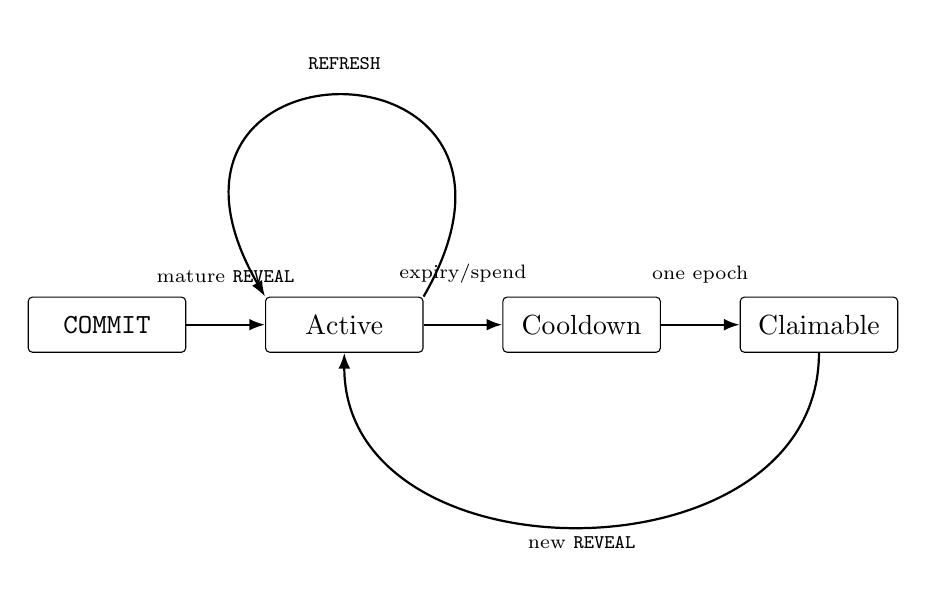
\begin{tikzpicture}[
  node distance=10mm and 10mm,
  state/.style={draw, rounded corners=1.5pt, minimum width=20mm,
                minimum height=7mm, align=center},
  flow/.style={-{Latex[length=2mm]}, thick},
  note/.style={font=\scriptsize, align=center}
]
\node[state] (commit) {\operation{COMMIT}};
\node[state, right=of commit] (active) {Active};
\node[state, right=of active] (cooldown) {Cooldown};
\node[state, right=of cooldown] (claimable) {Claimable};

\draw[flow] (commit) -- node[note, above=4mm] {mature \operation{REVEAL}} (active);
\draw[flow] (active) -- node[note, above=4mm] {expiry/spend} (cooldown);
\draw[flow] (cooldown) -- node[note, above=4mm] {one epoch} (claimable);
\draw[flow] (claimable.south) to[out=-90,in=-90,looseness=1.25]
  node[note, below] {new \operation{REVEAL}} (active.south);
\draw[flow] (active.north east) to[out=60,in=120,looseness=5]
  node[note, above=2mm] {\operation{REFRESH}} (active.north west);
\end{tikzpicture}
\caption{Coppice Names lifecycle. Acceptance of a \operation{REVEAL} also
requires the name window and a valid proof. A \operation{COMMIT} is not a
reservation.}
\label{fig:lifecycle}
\end{figure}

\section{Publication and discovery}

Names bulletins use Coppice application framing in zero-valued publication
carriers. The bond is a separate designated Ironwood action and is never held
or burned by a carrier.

\operation{COMMIT}s use the deployment's generic Coppice rendezvous route.
They reveal a commitment but not the target name. \operation{REVEAL} and
\operation{REFRESH} use a deterministic public route derived from the
deployment identifier and the name identifier. Anyone who knows a name can
derive the same route and inspect only the blocks in which that name is
eligible to operate.

This asymmetry serves two purposes:

\begin{itemize}
\item the initial commitment does not announce the target name before the
reveal; and
\item exact resolution does not require continuous acquisition of unrelated
generic-rendezvous traffic.
\end{itemize}

A \operation{REVEAL} carries an exact canonical reference to its historical
\operation{COMMIT}. The resolver fetches that one referenced compact
transaction, authenticates the corresponding full transaction and Ironwood
effects, and admits the \operation{COMMIT} atomically with the
\operation{REVEAL} block. A location supplied by an untrusted source is never
sufficient by itself.

\section{Deterministic schedule and lifecycle}

For activation height $A$, epoch length $E$, name window length $W$,
deployment identifier $D$, and name identifier $N$, the protocol derives one
offset:

\begin{align*}
H_N &= \operatorname{BLAKE2b\mbox{-}256}_{\texttt{CoppiceN2Off}}
       (D \parallel N), \\
\operatorname{offset}(N) &=
  \operatorname{LE64}(H_N[0..8]) \bmod (E-W+1), \\
\operatorname{window}(N,e) &=
  [A + eE + \operatorname{offset}(N),\;
    A + eE + \operatorname{offset}(N) + W).
\end{align*}

Intervals are half-open. \operation{REVEAL} and \operation{REFRESH} are
accepted only inside the name's window. A referenced \operation{COMMIT} must
have reached its maturity and must not have reached its TTL. Cheap schedule
and reference checks occur before proof verification.

The current candidate profiles are:

\begin{center}
\begin{tabular}{lrr}
\hline
Parameter & Production candidate & Regtest \\
\hline
Epoch & 1,152 blocks & 32 blocks \\
Name window & 24 blocks & 4 blocks \\
\operation{COMMIT} maturity & 24 blocks & 4 blocks \\
\operation{COMMIT} TTL & 192 blocks & 24 blocks \\
Lease & 250,000 blocks & 128 blocks \\
Cooldown & 1,152 blocks & 32 blocks \\
\hline
\end{tabular}
\end{center}

The production profile provides approximately daily operation opportunities
and a roughly six-month lease under the candidate timing assumption. Regtest
is intentionally accelerated and is cryptographically separated by its
deployment identifier. Production values remain \statusword{TBD} until
deployment.

When a bond is spent or a lease expires, the name enters a uniform one-epoch
cooldown during which it resolves to no payment address and no replacement can
be installed. This deliberately visible non-resolving interval reduces the
risk that a recently terminated name immediately begins paying a new owner.
The rule does not distinguish voluntary release from natural expiry, and the
former owner receives no special reclaim priority.

\section{Hidden ownership and zero-knowledge proofs}

The registrant's per-name Orchard authority is never published. The protocol
uses two fixed Halo2 proof statements, instantiated with an IPA polynomial
commitment over the Pasta curves~\cite{halo2-ipa}.

\subsection{REVEAL proof}

The prover opens the referenced \operation{COMMIT} and demonstrates that it
binds the deployment, name, target epoch, hidden owner commitment, and a
nonzero secret. The proof also establishes that the designated successor
action creates a note controlled by that hidden authority with value exactly
1 ZEC. Its public statement binds the canonical \operation{COMMIT} reference,
UA, inclusion epoch, action index, action nullifier and commitment, successor
future nullifier, and bond value.

\subsection{REFRESH proof}

The prover demonstrates that the designated predecessor and successor notes
both have value exactly 1 ZEC and are controlled by the same hidden authority.
The proof binds the accepted predecessor reference and commitment, its future
nullifier, the new canonical UA, the new epoch, and the successor action
effects. The reducer separately requires the predecessor to be the exact
current accepted head and the transaction to spend it.

Changing the UA and renewing without changing it are intentionally one
operation. Every accepted \operation{REFRESH} starts a full new lease from its
inclusion height. Transfer to a different hidden authority is not supported.

The current circuits use Halo2 IPA over the Pasta curves with $k=11$. Each
proof is 4,704 bytes. A deployment binds the generated verifying-key
fingerprint, parameter exponent, operation tag, and fixed proof length into its
verifier identity. Callers cannot select an alternate verifier.

The proofs establish private note relations; they do not replace canonical
history. Ordering, schedules, currentness, competing spends, and
reorganization handling remain deterministic public checks because those
facts arise from the chain rather than from the registrant's private witness.

\section{Canonical state and exact resolution}

Every resolver executes the same reducer over authenticated Zcash data. For
each transaction, it first records authenticated action nullifiers, then tries
to apply the decoded Names operation, and finally terminates any current head
spent by that transaction even if its bulletin was missing or invalid. This
prevents a proof-valid physical note from silently replacing accepted Names
state.

To resolve an arbitrary exact name, a client:

\begin{enumerate}
\item canonicalizes the label and derives its identifier, route, and eligible
windows;
\item authenticates candidate \operation{REVEAL} and \operation{REFRESH}
bulletins found in those windows;
\item follows a candidate \operation{REVEAL}'s bounded reference to its one
historical \operation{COMMIT};
\item applies proof, timing, routing, statement, and accepted-lineage checks;
and
\item observes authenticated Ironwood nullifiers through the relevant
canonical tail to determine whether the accepted head remains unspent and
active.
\end{enumerate}

An exact resolver and a complete replay must produce the same lifecycle,
record, head, and producer at the same canonical tip.

\subsection{Fast resolution without a trusted index}

The protocol cannot derive currentness from a signed database that maps names
to addresses: current Zcash consensus commits transaction history, not a
Coppice Names state root. A mutable local index therefore cannot become
authority simply because it records a plausible chain tip.

Instead, the wallet retains a rolling, branch-keyed window of authenticated
compact Ironwood evidence as part of ordinary Zcash synchronization.
Resolution still replays the deterministic rules locally, but it avoids
downloading the same six-month history on demand. The evidence store is derived
and reconstructible, follows normal wallet reorganization handling, and can be
evicted beyond the protocol horizon.

The wallet's existing Ironwood commitment tree also supplies authenticated
global action positions and tree-size transitions to Coppice. Names does not
maintain a duplicate commitment tree. The host checks pre- and post-scan tree
sizes and publishes candidate Names state only after the wallet's database
transaction commits.

This construction preserves arbitrary-name resolution and local verification
while moving the expensive work to the synchronization path the wallet already
performs.

\section{Wallet custody and recovery}

The bond remains an ordinary user-controlled shielded note. A supporting
wallet marks the exact 1 ZEC state note as managed so ordinary coin selection
does not spend it accidentally. That lock is wallet safety policy, not protocol
custody: the owner can explicitly release the name by spending the note.

The companion wallet policy derives, from the wallet seed:

\begin{itemize}
\item a Names master;
\item a deployment- and name-separated hidden spending authority;
\item deterministic epoch \operation{COMMIT} secrets; and
\item successor note material bound to canonical operation data.
\end{itemize}

The seed therefore recovers the secret authority. A nonsecret list of owned
names tells a restored wallet which exact names to test and recover. No fragile
sidecar secret is required, and importing one name does not require trusting a
bulk registry snapshot.

Recovery is explicit wallet behavior. Looking up an arbitrary name does not
silently attempt ownership recovery, and a wallet may expose recovery even
when other owned names are already present.

\section{Security analysis}

\subsection{Registration front-running}

\operation{COMMIT} hides the name and target opening before
\operation{REVEAL}. A copied \operation{REVEAL} cannot substitute another
hidden owner or successor note without satisfying the bound proof. A
\operation{COMMIT} does not reserve the name, so canonical ordering still
decides between independently valid competing registrations after the name
becomes claimable.

\subsection{Unauthorized update or release}

A \operation{REFRESH} must spend the exact current accepted predecessor and
prove the same hidden authority controls its successor. An attacker cannot
update the record using an older valid state. Release is the ordinary Zcash
spend of the current bond note and therefore requires its spending authority.

\subsection{Stale and shadow lineages}

Canonical \code{StateRef} and \code{CommitRef} values bind height,
transaction index, transaction identifier, and action index as applicable.
The reducer accepts only the exact current predecessor. Proof-valid notes on
rejected or stale branches cannot become Names authority merely by existing on
chain.

\subsection{Reorganizations}

Reducer snapshots and indexes are derived state. They are bound to deployment,
network, height, and canonical block hash and are rolled back with the wallet's
chain state. A block with the wrong height or previous hash is rejected. Deep
reorganizations beyond retained journals require reconstruction from
authenticated history rather than trusting the cached head.

\subsection{Malicious chain-data providers}

A provider can degrade availability, correlate selective requests, or present
the risks already present in the wallet's chain-source model. Coppice verifies
transaction identities, action effects, route selection, references, chain
continuity, and proofs before accepting an operation. A provider-supplied
name-to-UA answer is never protocol evidence.

\subsection{Resource exhaustion}

Candidate messages must pass inexpensive framing, route, schedule, reference,
transaction-shape, and lineage checks before proof verification. Exact
\operation{REVEAL} discovery never requires fetching unrelated generic-route
full transactions; only the historical \operation{COMMIT} explicitly
referenced by a candidate is acquired.

A targeted attacker can still publish traffic in a particular name's daily
window. The window bounds the affected blocks, while every candidate must be
published in a Zcash transaction, compete for block space, and ordinarily pay
the applicable Zcash fee under relay and mining policy~\cite{zip317}. Coppice
Names does not add transaction grinding: grinding complicates construction
without removing the targeted publication bound.

\subsection{Name impersonation after termination}

Cooldown prevents immediate reassignment after either expiry or explicit
release. During the interval the name resolves to no address, giving users and
applications a deterministic warning gap before a later registrant can install
a different record. It does not prove social identity and cannot prevent name
squatting or user confusion after the cooldown ends.

\subsection{Remaining assurance work}

Formal security definitions, proof sketches for uniqueness and accepted-head
agreement, an independent circuit review, and complete adversarial test
coverage are \statusword{WIP}. No claim of a completed independent audit is
made.

\section{Privacy analysis}

The design protects the registrant's hidden Orchard authority and hides the
target name during \operation{COMMIT}. Nevertheless, a naming protocol must
publish enough information for strangers to resolve a name.
\operation{REVEAL} and \operation{REFRESH} therefore publish the canonical
name, its UA, its schedule epoch, canonical references, and its name-derived
route. Operations for the same name are publicly linkable.

The designated state action is also linked to the public Names operation. Its
proof establishes the exact 1 ZEC bond relation, and its future spend
determines whether the name remains current. The authority and ordinary
shielded note plaintext remain hidden, but the application-level lineage is
intentionally observable.

Remote exact-window requests can reveal which name a client is resolving. A
rolling local evidence store reduces this leakage because normal wallet sync
acquires the canonical evidence before the lookup and does not need a
name-specific remote query. Private information can still leak through wallet
network behavior, transaction timing, UA receiver composition, or compromise
of the wallet itself.

Coppice Names offers privacy relative to public ownership registries and
trusted resolution services; it does not make public names or their payment
records secret.

\section{Economics and anti-spam}

Every active name immobilizes exactly 1 ZEC in a shielded note controlled by
the registrant. The value is refundable and is not a protocol fee. It imposes
a capital cost on maintaining many simultaneous names while preserving the
user's ownership of the funds.

\operation{COMMIT}, \operation{REVEAL}, \operation{REFRESH}, and release are
normal Zcash transactions to which the wallet applies Zcash fee policy. Those
fees, relay policy, and Zcash block limits are the publication anti-spam
mechanism; Coppice Names does not burn ZEC, levy rent, or create a separate fee
market. The fixed bond and transaction fees play different roles and must not
be conflated.

The wallet may display 1 ZEC as bonded rather than spendable while the name is
active. An explicit release returns the note's value to ordinary wallet
control minus the transaction fee.

\section{Performance evaluation}

The current evaluation uses a retained 250,000-block mainnet workload covering
heights 3,220,327 through 3,470,326. Pre-NU6.3 Orchard compact actions and
post-NU6.3 Ironwood compact actions are treated as one Orchard-family workload
for action density and byte-volume measurement. They are not presented as a
comparison between the two pools.

\subsection{Historical workload}

\begin{center}
\small
\begin{tabular}{>{\raggedright\arraybackslash}p{0.57\textwidth}r}
\hline
Quantity & Observed value \\
\hline
Blocks & 250,000 \\
Orchard-family actions & 688,370 \\
Action-bearing transactions & 276,271 \\
Compact protobuf payload & 143.14 MB \\
Mean actions per block & 2.753 \\
Payload per block, p50 / p95 / p99 & 448 / 1,876 / 3,427 bytes \\
Sequential acquisition time in retained capture & 67.96 s \\
\hline
\end{tabular}
\end{center}

Matched endpoint samples later produced a median observed payload throughput
of 0.892 MB/s and median request overhead of 265 ms. Applying that calibration
to a six-month full-tail reacquisition gives 160.4 seconds at baseline traffic.
This is a \statusword{modeled} acquisition value, not a service-level
guarantee.

\subsection{Wallet-owned position replay}

\begin{center}
\small
\begin{tabular}{>{\raggedright\arraybackslash}p{0.57\textwidth}rr}
\hline
Replay path & Time & Evidence class \\
\hline
Reference Coppice components with duplicate tree work & 239.519 s & Measured \\
Production \code{CorePositionRuntime} plus Names & 1.853 s & Measured \\
Independent tree-free confirmation consumer & 1.706 s & Measured \\
\hline
\end{tabular}
\end{center}

The production path reduced measured Coppice component time by 99.23\%. It
matched every global action position and block tree-size transition, matched
wallet/Core roots at 250 fixed checkpoints and the final tip, reached the same
688,370-leaf root, and reproduced the final state after rolling back and
reapplying the last block.

This benchmark isolates in-memory replay. It excludes wallet SQLite cost,
network transfer, routed full transactions, Names proof verification on live
Coppice traffic, and a live multi-block replacement-branch reorganization.
Those exclusions prevent treating 1.853 seconds as an end-to-end user latency.

\subsection{Arbitrary-name lookup choices}

At baseline traffic, the current model gives:

\begin{center}
\small
\begin{tabular}{>{\raggedright\arraybackslash}p{0.43\textwidth}>{\raggedleft\arraybackslash}p{0.18\textwidth}>{\raggedright\arraybackslash}p{0.21\textwidth}}
\hline
Evidence strategy & Six-month cost & Classification \\
\hline
Reacquire full compact tail remotely & 160.4 s & Modeled \\
Fetch nullifier effects plus 218 separate name windows & 61.2 s & Modeled \\
Traverse retained local compact evidence & 0.224 s raw decode & Measured component \\
Production Core-position plus Names replay & 1.853 s & Measured component \\
\hline
\end{tabular}
\end{center}

The sparse remote strategy downloads fewer bytes but pays round-trip overhead
for many disjoint windows and creates more observable query behavior. The
preferred path retains approximately 143 MB of rolling compact evidence in the
measured baseline and resolves locally. A sparse nullifier journal plus
\operation{COMMIT} tail remains a lower-storage fallback, not the default fast
path.

\subsection{Synthetic adoption loads}

Synthetic, non-consensus Names-shaped transactions were inserted into a copy
of the historical workload at declared rates. A default synthetic transaction
contains 13 Orchard-family actions, matching the qualified transport shape but
not claiming to be a valid mainnet Coppice transaction.

\begin{center}
\small
\begin{tabular}{rrrr}
\hline
Names tx/day & Six-month payload & Raw decode & Modeled acquisition \\
\hline
0 & 143.14 MB & 0.224 s & 160.4 s \\
10 & 147.71 MB & 0.237 s & 165.5 s \\
100 & 188.91 MB & 0.311 s & 211.7 s \\
1,000 & 600.82 MB & 0.974 s & 673.3 s \\
\hline
\end{tabular}
\end{center}

The experiment indicates that evidence acquisition, rather than protobuf
decoding, dominates cold lookup across the modeled range. Synthetic results
describe scaling behavior and are not adoption forecasts.

\subsection{Adversarial load}

Under an intentionally extreme 2 MB block-fill model, continuous generic-route
acquisition could cause roughly 40.5 million unrelated full-transaction
fetches, 499 GB of data, and 39.9 hours of local route processing over six
months. The exact referenced-\operation{COMMIT} design reduces unrelated
generic full-transaction fetches during exact resolution to zero.

A targeted attacker can instead fill one name's 24-block window. The current
model bounds that window at approximately 1,080 reveal-shaped candidates and
21.34 seconds of route plus invalid-proof CPU, in addition to the attacker's
need to publish referenced \operation{COMMIT}s and pay Zcash fees. This is a
conservative modeled ceiling, not a measured live attack.

\subsection{Evaluation limits}

Before deployment, the following measurements remain \statusword{WIP}:

\begin{itemize}
\item complete wallet lookup latency including SQLite and UI;
\item proof generation and verification for actual V6 13-action Names
transactions;
\item live routed full-transaction acquisition;
\item restart and cache-reconstruction latency for owned names;
\item replacement-branch reorganization under managed note insertion; and
\item multi-device and multi-provider availability behavior.
\end{itemize}

The retained corpus, deterministic synthetic generator, raw results, model,
and charts form the current reproducibility package. The generator and model
live in the \href{https://github.com/nfl0/zcash-devtool}{zcash-devtool} repository. A
stable public archive of the retained corpus and a citation identifier are
\statusword{TBD}.

\section{Conformance and deployment}

The checked-in positive conformance artifact freezes the deployment, verifier
suite, route derivation, schedule, statements, real proofs, operation encoding,
and resolved heads. Rust and independent Python consumers verify the same
artifact. Negative tests reject malformed encodings, wrong routes and
networks, stale predecessors, invalid timing, wrong action indexes, proof
substitution, wrong bond values, noncanonical order, and wrong-branch
snapshots.

Conformance does not substitute for deployment qualification. Before a
production activation, the project must finalize the production parameter set
and verifier identities, publish reproducible artifacts, complete independent
review, and exercise the complete lifecycle and reorganization behavior over a
representative live environment. The production activation height is
\statusword{TBD}.

\section{Limitations and open work}

Coppice Names deliberately accepts several limitations:

\begin{itemize}
\item Names and UAs are public after \operation{REVEAL}.
\item Exact remote queries can leak lookup interest unless evidence is acquired
by ordinary wallet sync.
\item A resolver must retain or reacquire canonical evidence; Zcash consensus
does not provide a Names state commitment.
\item A fixed 1 ZEC bond limits accessibility when ZEC's purchasing power
changes.
\item Daily operation windows intentionally make record updates and renewals
non-instantaneous.
\item Cooldown sacrifices immediate reuse to reduce abrupt impersonation risk.
\item The protocol proves control, not legal or social identity.
\item Name transfer is unsupported.
\end{itemize}

Open engineering and assurance work is listed as WIP rather than silently
assumed complete. Future investigation may improve circuits, proof costs,
storage layout, or acquisition privacy, but any change must preserve arbitrary
resolution, canonical replay, hidden authority, and the absence of a trusted
resolver.

\section{Conclusion}

Coppice Names turns the Zcash chain into a privacy-aware naming substrate
without asking Zcash consensus to understand names. A refundable shielded bond
represents continuing control; zero-knowledge proofs validate private
ownership transitions; deterministic replay validates public protocol state;
and name-derived routes make arbitrary resolution practical.

The principal performance result is architectural rather than merely an
implementation optimization: wallets should retain canonical evidence during
their ordinary scan and let Names reuse wallet-owned commitment-tree facts.
That keeps resolution local, fast, and independently verifiable without
promoting a third-party service or mutable local index into protocol authority.

\begin{thebibliography}{9}

\bibitem{zcash-protocol}
The Electric Coin Company and Zcash contributors.
\newblock \emph{Zcash Protocol Specification}.
\newblock \url{https://zips.z.cash/protocol/protocol.pdf}.

\bibitem{zip258}
Zcash Improvement Proposal 258.
\newblock \emph{Deployment of the NU6.3 Network Upgrade}.
\newblock \url{https://zips.z.cash/zip-0258}.

\bibitem{zip229}
Zcash Improvement Proposal 229.
\newblock \emph{Version 6 Transaction Format}.
\newblock \url{https://zips.z.cash/zip-0229}.

\bibitem{zip316}
Zcash Improvement Proposal 316.
\newblock \emph{Unified Addresses and Unified Viewing Keys}.
\newblock \url{https://zips.z.cash/zip-0316}.

\bibitem{zip317}
Zcash Improvement Proposal 317.
\newblock \emph{Proportional Transfer Fee Mechanism}.
\newblock \url{https://zips.z.cash/zip-0317}.

\bibitem{zip318}
Zcash Improvement Proposal 318.
\newblock \emph{Orchard to Ironwood Migration}.
\newblock \url{https://zips.z.cash/zip-0318}.

\bibitem{zip326}
Zcash Improvement Proposal 326.
\newblock \emph{NU6.3 Consequences for Wallets}.
\newblock \url{https://zips.z.cash/zip-0326}.

\bibitem{halo2-ipa}
The halo2 contributors.
\newblock \emph{Polynomial commitment using an inner product argument}.
\newblock \url{https://zcash.github.io/halo2/background/pc-ipa.html}.

\end{thebibliography}

\end{document}
